\documentclass{article}

\usepackage{amsthm}
\usepackage{amsfonts}
\usepackage{amsmath}
\usepackage{amssymb}
\usepackage{fullpage}
\usepackage{graphicx}
\usepackage[usenames]{color}
\usepackage{hyperref}
\usepackage{graphicx}
\usepackage{stmaryrd}
\usepackage{float}
\usepackage{amsmath}




  \hypersetup{
    colorlinks = true,
    urlcolor = blue,       
    linkcolor= blue,      
    citecolor= blue,      
    filecolor= blue,     
    }
    
\usepackage{listings}

\definecolor{dkgreen}{rgb}{0,0.6,0}
\definecolor{gray}{rgb}{0.5,0.5,0.5}
\definecolor{mauve}{rgb}{0.58,0,0.82}

\lstset{frame=tb,
  language=haskell,
  aboveskip=3mm,
  belowskip=3mm,
  showstringspaces=false,
  columns=flexible,
  basicstyle={\small\ttfamily},
  numbers=none,
  numberstyle=\tiny\color{gray},
  keywordstyle=\color{blue},
  commentstyle=\color{dkgreen},
  stringstyle=\color{mauve},
  breaklines=true,
  breakatwhitespace=true,
  tabsize=3
}

\theoremstyle{plain} 
   \newtheorem{theorem}{Theorem}[section]
   \newtheorem{corollary}[theorem]{Corollary}
   \newtheorem{lemma}[theorem]{Lemma}
   \newtheorem{proposition}[theorem]{Proposition}
\theoremstyle{definition}
   \newtheorem{definition}[theorem]{Definition}
   \newtheorem{example}[theorem]{Example}
\theoremstyle{remark}    
  \newtheorem{remark}[theorem]{Remark}

\title{CPSC 354 Report}
\author{Andrew Eppich  \\ Chapman University}
\date{\today}

\begin{document}

\maketitle

\begin{abstract}

\end{abstract}

\tableofcontents

\section{Introduction}\label{intro}

\section{Homework 1}\label{homework1}

\subsection{Question 5}

\begin{lstlisting}
rw [add_zero]
rw [add_zero]
rfl
\end{lstlisting}

\subsubsection{Proof Explanation}

For this question, the Lean proof is related to the corresponding proof in mathematics because we know that we can use the additive identity property, which says that \(x + 0 = x\). By using this, we can simplify \(b + 0\) and \(c + 0\) easily to get \(a + b + c = a + b + c\), which we can determine is the same by the reflexivity property, which states that if \(a = b\), then \(a\) and \(b\) are identical. Therefore, \(a + b + c\) is identical to \(a + b + c\).

\subsection{Question 6}

\begin{lstlisting}
rw [add_zero c]
rw [add_zero b]
rfl
\end{lstlisting}


\subsection{Question 7}

\begin{lstlisting}
rw [one_eq_succ_zero]
rw [add_succ]
rw [add_zero]
rfl
\end{lstlisting}


\subsection{Question 8}

\begin{lstlisting}
rw [two_eq_succ_one]
rw [one_eq_succ_zero]
rw [add_succ]
rw[add_succ]
rw [add_zero]
rw [four_eq_succ_three]
rw [three_eq_succ_two]
rw [two_eq_succ_one]
rw [one_eq_succ_zero]
rfl
\end{lstlisting}

\subsection{Discord Question}

I was wondering if the computers use of discrete math extends to all program computations or just math computations

\section{Homework 2}\label{homework2}

\subsection{Question 1}

\begin{lstlisting}
induction n with d hd
rw [add_zero]
rfl
rw [add_succ]
rw [hd]
rfl
\end{lstlisting}

\subsection{Question 2}

\begin{lstlisting}
  induction b with d hd
  rw [add_zero]
  rw [add_zero]
  rfl
  rw [add_succ]
  rw [add_succ]
  rw [hd]
  rfl
\end{lstlisting}

\subsection{Question 3}

\begin{lstlisting}
induction b with d hd
rw [add_zero]
rw [zero_add]
rfl
rw [add_succ]
rw [hd]
rw [succ_add]
rfl
\end{lstlisting}

\subsection{Question 4}

\begin{lstlisting}
  induction a with d hd
  rw [zero_add]
  rw [zero_add]
  rfl
  rw [succ_add]
  rw [succ_add]
  rw [succ_add]
  rw [hd]
  rfl
\end{lstlisting}

\subsubsection{Explaination}

The lean proof relates to the proof in mathematics because it uses induction to solve the problem. Then the Lean proof is solved by solving the equation of the successors. Just like in mathematics it uses simple rules to change the positioning of the parenthesis so each side is exactly the same. This is exactly like how the mathematical proof would be written.

\subsection{Question 5}

\begin{lstlisting}
  induction a with d hd
  rw [zero_add]
  rw [zero_add]
  rw [add_comm]
  rfl
  rw [add_comm]
  rw [add_comm]
  rw [succ_add]
  rw [succ_add]
  rw [succ_add]
  rw [succ_add]
  rw [hd]
  rfl
\end{lstlisting}

\subsection{Discord Question}

I was wondering how discrete math and the recursive algorithms we talked about fit into a programming language and how it actually works

\section{Homework 3}\label{homework3}

\subsection{Discord Post}

Discord Name: Andrew Eppich.   
In my literature review with ChatGPT, I explored interpreted vs. compiled programming languages. I found that interpreted languages are changed from user to machine code line by line, which is inefficient. Compiled languages are compiled from user to machine code all at once and then run which makes it faster and easier to spot errors. From there I explored interpreted languages and their role in machine learning as well as their history in machine learning. I first found that compiled was much more efficient than interpreted. I then found out that interpreted is mainly used for machine learning. It is mainly used because of the extensive amount of libraries used with interpreted languages, especially Python. Some of those libraries include NumPy, pandas, scikit-learn, TensorFlow, and Matplotlib. These libraries are crucial for machine learning because they are associated with data processing and deep learning. I then took a look into the history of programming languages with machine learning. I found that at first compiled languages were used from the 1950s-1980s. In 1991, Python was developed which became the standard for machine learning in the early 2000s. Python became the main language for machine learning from 2010 and on because of its libraries TensorFlow and PyTorch. 
\url{https://github.com/AndrewEppich/LLM-Literature-Review/blob/main/README.md}

\subsection{Reports Voted For}

\url{https://github.com/zackklopukh/LLMReport}

\url{https://github.com/maxler0y/354_HW3}

\section{Homework 4}\label{homework4}

\begin{figure}[H]
  \centering
  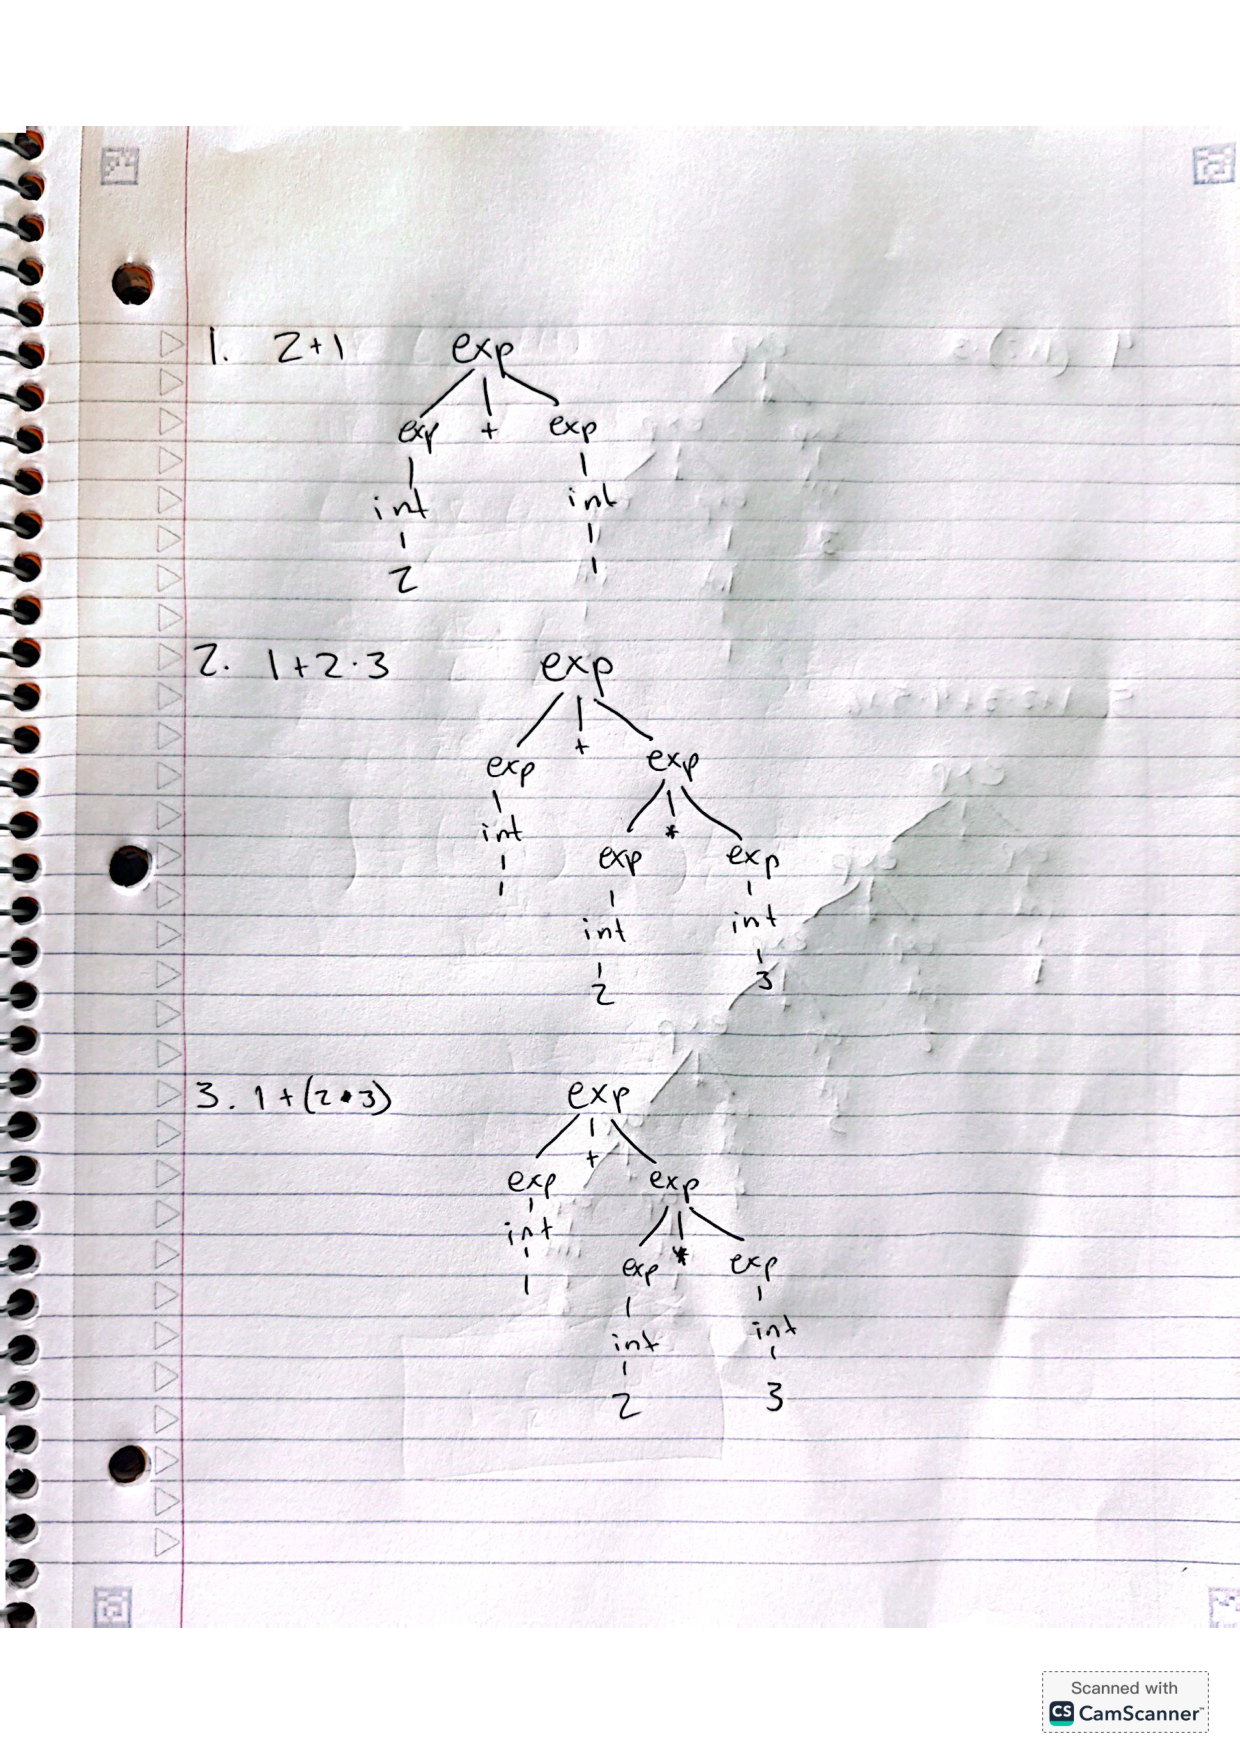
\includegraphics[width=0.7\textwidth, page=1]{CPSC_354_Homework_4.pdf}
  \caption{Homework 4 - Page 1}
  \label{fig:homework4_page1}
\end{figure}

\begin{figure}[H]
  \centering
  \includegraphics[width=0.7\textwidth, page=2]{CPSC_354_Homework_4.pdf}
  \caption{Homework 4 - Page 2}
  \label{fig:homework4_page2}
\end{figure}

\subsection{Discord Question}

How complex do parsing algorithms get the farther down the level of programming languages you go?


\section{Homework 5}\label{homework5}

\subsection{Question 1}

\begin{lstlisting}
  exact todo_list
\end{lstlisting}

\subsection{Question 2}

\begin{lstlisting}
  exact and_intro p s
\end{lstlisting}

\subsection{Question 3}

\begin{lstlisting}
  exact <a,i>, <o,u>
\end{lstlisting}

\subsection{Question 4}

\begin{lstlisting}
  have p := vm.left
  exact p
\end{lstlisting}

\subsection{Question 5}

\begin{lstlisting}
  exact and_right h
\end{lstlisting}

\subsection{Question 6}

\begin{lstlisting}
  have a:= and_left h1
  have b := and_right h2
  exact < a, b>
\end{lstlisting}

\subsection{Question 7}

\begin{lstlisting}
  have h1 := h.right
  have h2 := h.left
  have h3 := h2.right
  exact h.left.right.left.left.right
\end{lstlisting}

\subsection{Question 8}

\begin{lstlisting}
  have h1 := and_left h
  have h2 := and_right h
  have h3 := and_right h2
  have h4 := and_left h3
  have h5 := and_left h4
  have h6 := and_right h1
  have h7 := and_left h1
  have h8 := and_left h7
  have h9 := and_right h7
  exact < h6, h5, h8, h9>
\end{lstlisting}

\subsubsection{Proof Explaination}
I took the left and right sides and set them equal to different variables. Next I took those broken down parts and continued to break them down into different variables until I had a single value for a single variable. Then I added the desired variables together to acheive the desired equation

\subsection{Discord Question}
When thinking about the final Lean problem on the homework, I solved it by breaking up each term over and over again with and\_left and and\_right until there were single terms. It was like a tree forming a new branch and leaves every time the equation was broken up. My question is, how is the logic of AND and and\_left and and\_right used in programming languages and other applications? And is this just the logic that is used to parse a BST?	

\section{Homework 6}\label{homework6}

\subsection{Lecture Explaination}

\begin{lstlisting}
In lecture this week we started learning about lambda caclulus. We learned about the syntax of P -> Q. We learned about the rule of how to eliminate so we can prove P -> Q by saying P is evidence of B so h \( A \) :B. We also learned that we can use lambda to create a function of terms that is able to be broken apart. We alsp learned the transitive property that says \( P -> Q \) -> \( Q -> R \) -> P -> R.
\end{lstlisting}

\subsection{Question 1}

\begin{lstlisting}
exact bakery_service p
\end{lstlisting}

\subsection{Question 2}

\begin{lstlisting}
  have h1 : C -> C := fun C \mapsto C
  exact h1
  \end{lstlisting}
  
  \subsection{Question 3}
  
  \begin{lstlisting}
    exact fun h : I \mapsto and_intro (and_right h) h.left
    \end{lstlisting}


\subsection{Question 4}

\begin{lstlisting}
exact fun c => h2 (h1 c)
\end{lstlisting}

\subsection{Question 5}

\begin{lstlisting}
have q : Q := h1 p
have t : T := h3 q
exact h5 t
\end{lstlisting}

\subsection{Question 6}

\begin{lstlisting}
exact fun c => fun d => h <c, d>
\end{lstlisting}

\subsection{Question 7}

\begin{lstlisting}
exact fun h1 => h h1.1 h1.2
\end{lstlisting}

\subsection{Question 8}

\begin{lstlisting}
exact fun s => < h.1 s, h.2 s>
\end{lstlisting}

\subsection{Question 9}

\begin{lstlisting}
exact fun r => < fun s => r, fun ns => r>
\end{lstlisting}

\subsection{Discord Question}

are lambda calculus proofs a part of the compiler? if so, how do they interact with the code that is being compiled?


\section{Homework 7}\label{homework7}

\subsection{Question 1}

\textbf{Beta Reduction 1:}
\[
((\lambda m. \lambda n. m \, n) \, (\lambda f. \lambda x. f(f \, x))) \, (\lambda f. \lambda x. f(f(f \, x)))
\]

\textbf{Beta Reduction 2:}
\[
\lambda n. (\lambda f. \lambda x. f(f \, x)) \, n
\]

\textbf{Beta Reduction 3:}
\[
(\lambda f. \lambda x. f(f \, x)) \, (\lambda f. \lambda x. f(f(f \, x)))
\]

\textbf{Beta Reduction 4:}
\[
\lambda x. (\lambda f. \lambda x. f(f(f \, x))) \, (\lambda f. \lambda x. f(f(f \, x)) \, x)
\]

\textbf{Beta Reduction 5:}
\[
\lambda x. (\lambda x. f(f(f(f(f \, x))))) \, ((\lambda f. \lambda x. f(f(f \, x))) \, x)
\]

\textbf{Beta Reduction 6:}
\[
\lambda x. f(f(f(f(f(f \, x)))))
\]

\textbf{Beta Reduction 7:}
\[
\lambda x. f(f(f(f(f(f(f \, x))))))
\]


\subsection{Question 2}

The function takes two Church numerals m and n and applies m to n. Applying m to n is like multiplying two numbers so it implements multiplication

\subsection{Discord Questions}

how complex does lambda calculus recursion get in computer systems?


\section{Homework 8-9}\label{homework89}

\subsection{Question 2}

  a b c d reduces to that because in the code it parses the expression and characterizes it as app which is in the lark grammar defined as exp1 exp2 so it takes a and b and puts parenthesis around it. Then it goes to the next expression whcih is /(a + b /) and then gets the next term which is c so it puts parenthesis around /(a + b /) and c. Then it does this process again with d. then if you have /(a/) it will just return a because in lark grammar it is characterized as var. In the code if the expression is var it returns just the term in the parenthesis so it just returns a

\subsection{Question 3}

Capture avoiding subsittuion works because when when substituting variables, if there is a free variable in the expression then substituting variables in the equation can cause the expression to change its meaning. Capture-avoiding substitutions avoid capturing free variables in the expression when changing a variable which can cause the whole expression to change its meaning. in the code it checks bound variable matches the substitution target, if it does it leaves it unchanged if not it generates a new variable

\subsection{Question 4}

We do not always get the expected results. Well-defined expressions typically return the expected results, but if there is an error handling an edge case, it would not return the expected results. Not all computations reduce to normal form. Expressions like \((\lambda x. \, x \, x)\) and \((\lambda x. \, x \, x)\) create an infinite loop of self-application that will never be stable.

\subsection{Question 5}

This is the smallest lambda function that doesn’t reduce to normal form: \((\lambda x. \, x \, x) \, (\lambda x. \, x \, x)\). This reduces to itself, so there is no normal form.

\subsection{Quesdtion 7}

\textbf{Initial Expression}:
\[
((\lambda m.\, \lambda n.\, m \, n) \, (\lambda f.\, \lambda x.\, f \, (f \, x))) \, (\lambda f.\, \lambda x.\, f \, (f \, (f \, x)))
\]

\textbf{First Application}:
Apply \((\lambda m.\, \lambda n.\, m \, n)\) to \((\lambda f.\, \lambda x.\, f \, (f \, x))\):
\[
(\lambda n.\, (\lambda f.\, \lambda x.\, f \, (f \, x)) \, n)
\]

\textbf{Second Application}:
Now apply \((\lambda n.\, (\lambda f.\, \lambda x.\, f \, (f \, x)) \, n)\) to \((\lambda f.\, \lambda x.\, f \, (f \, (f \, x)))\), substituting \(n\) with \((\lambda f.\, \lambda x.\, f \, (f \, (f \, x)))\):
\[
(\lambda f.\, \lambda x.\, f \, (f \, x)) \, (\lambda f.\, \lambda x.\, f \, (f \, (f \, x)))
\]

\textbf{Evaluating the Final Application}:
Substitute \((\lambda f.\, \lambda x.\, f \, (f \, (f \, x)))\) for \(f\) in \((\lambda f.\, \lambda x.\, f \, (f \, x))\):
\[
\lambda x.\, ((\lambda f.\, \lambda x.\, f \, (f \, (f \, x))) \, x)
\]

\textbf{Result}:
The final expression (in normal form) is:
\[
\lambda x.\, (\lambda f.\, \lambda x.\, f \, (f \, (f \, x))) \, x
\]

\subsection{Question 8}

\begin{verbatim}
  12: evaluate(((\m.\n. m n) (\f.\x. f (f x))) (\f.\x. f x))
      39: evaluate((\m.\n. m n) (\f.\x. f (f x)))
          12: evaluate(\m.\n. m n) = \m.\n. m n
          12: evaluate(\f.\x. f (f x)) = \f.\x. f (f x)
          51: substitute(\n. m n, m, (\f.\x. f (f x)))
              51: substitute((\f.\x. f (f x)) n, n, (\f.\x. f x))
          12: evaluate((\n. (\f.\x. f (f x)) n))
              51: substitute((\f.\x. f (f x)) n, n, (\f.\x. f x))
      39: evaluate((\f.\x. f (f x)) (\f.\x. f x))
          51: substitute((\x. f (f x)), f, (\f.\x. f x))
              51: substitute((\x. ((\f.\x. f x) ((\f.\x. f x) x))), f, (\f.\x. f x))
  \end{verbatim}

\subsection{Discord Questions}

Week 8: What does it mean in terms of a programming language output when something does not reduce to normal form

Week 9: how often is tracing used in the debugger in industry


\section{Homework 10}\label{homework10}

1. I found that figuring out the debugger and how to use the print statements like print(linearize(x)) was the hardest aspect because it took a while for me to get it to work

2. I came up with the key insight because I was struggling to figure out how to make sure the MWE returned the correct result. I figured out that if the expressions were identical then the result would be the same as the expressions. So i added a part that checked for that

3. The most interesting takeaway from this was learning how to use code to evaluate the lambda expressions

\subsection{Discord Question}

week 10: what aspects if coding prompts substitutions to be made to evaluate it

\section{Homework 11}\label{homework11}

\begin{figure}[H]
  \centering
  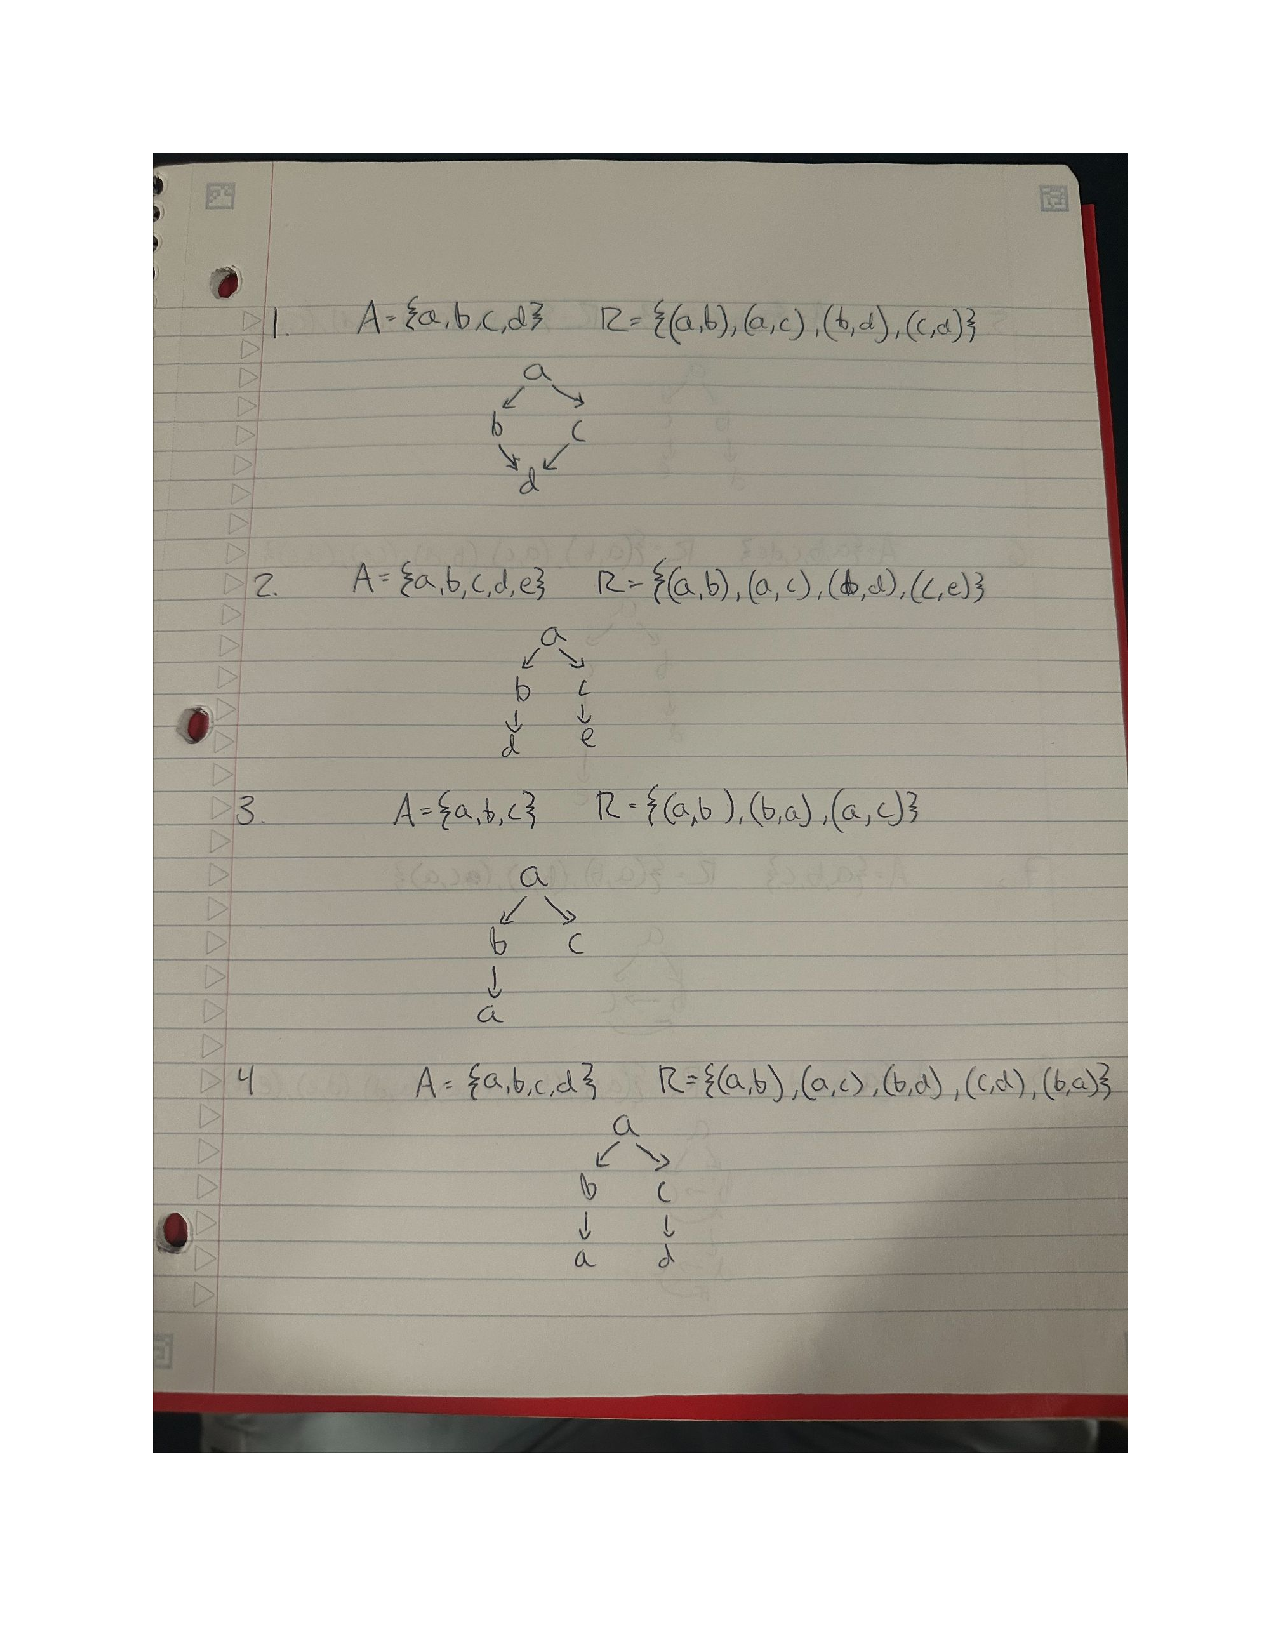
\includegraphics[width=0.7\textwidth, page=1]{HW11.pdf}
  \caption{Homework 11 - Page 1}
  \label{fig:homework11_page1}
\end{figure}

\begin{figure}[H]
  \centering
  \includegraphics[width=0.7\textwidth, page=2]{HW11.pdf}
  \caption{Homework 11 - Page 2}
  \label{fig:homework11_page2}
\end{figure}


\subsection{Discord Question}

If an ARS is not terminating is that a similar situation to when code has an infinite loop


\section{Homework 12}\label{homework12}

\subsection{Exercise 1}

* The ARS terminates because it is reduced to a unique form 
* The result of the computation is ab, which is the sorted version of the original
* It is unique because it is sorted so it can not be reduced anymore
* This algorithm implements bubble sort

\subsection{Exercise 2}

* The ARS terminates because it cannot be reduced any more
* The normal forms are a and b
* There is no string that will reduce to a and b, there have to be an even number of a to reduce to a but there have to be an odd number of b to reduce to a
* It is confluent because all reductions lead to a unique normal form
* If you replace -> with = then aa = bb and ab = ba
* The expression is equal to a when there is an even number of bs and equal to be if there are an odd number of bs
* Even count of bs → a, odd count of bs → b
* The algorithm computes whether there is an odd or even amount of bs

\subsection{Exercise 3}

* The algorithm does not terminate because when ba -> ab and ab -> ba so there is an infinite loop of reduction
* There are no normal forms because it does not terminate
* Change ab → ba to ab → b
* The algorithm removes duplicates from the string

\subsection{Exercise 4}

* The ARS does not terminate because ab → ba and ba → ab makes an infinite loop
* There are no normal forms because it does not terminate
* The results are not confluent because they do not reduce to a unique result
* This algorithm allows a and b to be switched to find all permutations of sequences with ab

\subsection{Exercise 5}

* abba → abba , bababa → bababa
* It is not terminating because ab → ba and ba → ab allow looping
* One class for each combination of counts of as and bs, there are no normal forms
* You can modify ba → ab to ba → b
* One question you can answer using this ARS is if two strings are equivalent 

\subsection{Exercise 5b}

* abba → abba, bababa → bababa
* It does not terminate because ab → ba and ba → ab allow for infinite looping
* The equivalence classes are the count of as modulo 2, and complete removal of bs the 
* Normal forms are both a
* Is the parity of as preserved in the equivalence class

\subsection{Discord Question}

what other uses do ARSs have besides sorting strings and how are they implemented 


\section{Homework 13}\label{homework13}

\[
\text{let rec } \mathit{fact} = \lambda n. \text{ if } n = 0 \text{ then } 1 \text{ else } n \cdot \mathit{fact}(n-1) \text{ in } \mathit{fact}(3)
\]
\[
\to \text{\textbf{<def of let rec>}} \quad \mathit{fact} = \mathit{fix} \, F, \text{ where } F = \lambda f. \lambda n. \text{if } n = 0 \text{ then } 1 \text{ else } n \cdot f(n-1)
\]
\[
\to \mathit{fix} \, F \, 3 \quad \text{\textbf{<def of fix>}}
\]
\[
\to F(\mathit{fix} \, F) \, 3 \quad \text{\textbf{<beta rule: substitute } F\text{>}}
\]
\[
\to (\lambda f. \lambda n. \text{if } n = 0 \text{ then } 1 \text{ else } n \cdot f(n-1))(\mathit{fix} \, F) \, 3
\]
\[
\to \lambda n. \text{if } n = 0 \text{ then } 1 \text{ else } n \cdot (\mathit{fix} \, F)(n-1) \quad \text{\textbf{<beta rule>}}
\]
\[
\to \text{if } 3 = 0 \text{ then } 1 \text{ else } 3 \cdot (\mathit{fix} \, F)(3-1) \quad \text{\textbf{<beta rule: substitute } 3\text{>}}
\]
\[
\to 3 \cdot (\mathit{fix} \, F)(2) \quad \text{\textbf{<def of if>}}
\]
\[
\to 3 \cdot F(\mathit{fix} \, F)(2) \quad \text{\textbf{<def of fix>}}
\]
\[
\to 3 \cdot (\lambda f. \lambda n. \text{if } n = 0 \text{ then } 1 \text{ else } n \cdot f(n-1))(\mathit{fix} \, F)(2) \quad \text{\textbf{<beta rule>}}
\]
\[
\to 3 \cdot (\lambda n. \text{if } n = 0 \text{ then } 1 \text{ else } n \cdot (\mathit{fix} \, F)(n-1))(2) \quad \text{\textbf{<beta rule>}}
\]
\[
\to 3 \cdot (\text{if } 2 = 0 \text{ then } 1 \text{ else } 2 \cdot (\mathit{fix} \, F)(2-1)) \quad \text{\textbf{<beta rule: substitute } 2\text{>}}
\]
\[
\to 3 \cdot (2 \cdot (\mathit{fix} \, F)(1)) \quad \text{\textbf{<def of if>}}
\]
\[
\to 3 \cdot (2 \cdot F(\mathit{fix} \, F)(1)) \quad \text{\textbf{<def of fix>}}
\]
\[
\to 3 \cdot (2 \cdot (\lambda f. \lambda n. \text{if } n = 0 \text{ then } 1 \text{ else } n \cdot f(n-1))(\mathit{fix} \, F)(1)) \quad \text{\textbf{<beta rule>}}
\]
\[
\to 3 \cdot (2 \cdot (\lambda n. \text{if } n = 0 \text{ then } 1 \text{ else } n \cdot (\mathit{fix} \, F)(n-1))(1)) \quad \text{\textbf{<beta rule>}}
\]
\[
\to 3 \cdot (2 \cdot (\text{if } 1 = 0 \text{ then } 1 \text{ else } 1 \cdot (\mathit{fix} \, F)(1-1))) \quad \text{\textbf{<beta rule: substitute } 1\text{>}}
\]
\[
\to 3 \cdot (2 \cdot (1 \cdot (\mathit{fix} \, F)(0))) \quad \text{\textbf{<def of if>}}
\]
\[
\to 3 \cdot (2 \cdot (1 \cdot F(\mathit{fix} \, F)(0))) \quad \text{\textbf{<def of fix>}}
\]
\[
\to 3 \cdot (2 \cdot (1 \cdot (\lambda f. \lambda n. \text{if } n = 0 \text{ then } 1 \text{ else } n \cdot f(n-1))(\mathit{fix} \, F)(0))) \quad \text{\textbf{<beta rule>}}
\]
\[
\to 3 \cdot (2 \cdot (1 \cdot (\lambda n. \text{if } n = 0 \text{ then } 1 \text{ else } n \cdot (\mathit{fix} \, F)(n-1))(0))) \quad \text{\textbf{<beta rule>}}
\]
\[
\to 3 \cdot (2 \cdot (1 \cdot (\text{if } 0 = 0 \text{ then } 1 \text{ else } 0 \cdot (\mathit{fix} \, F)(0-1)))) \quad \text{\textbf{<beta rule: substitute } 0\text{>}}
\]
\[
\to 3 \cdot (2 \cdot (1 \cdot 1)) \quad \text{\textbf{<def of if>}}
\]
\[
\to 3 \cdot (2 \cdot 1) = 3 \cdot 2 = 6 \quad \text{\textbf{<combine results>}}
\]
\[
\text{Final Result: } \mathit{fact}(3) = 6
\]



\end{document}
